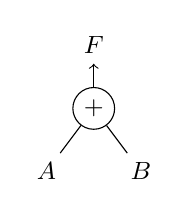
\begin{tikzpicture}[
    gate/.style={circle, draw, inner sep=2pt},
    every node/.style={font=\small}
]

% Inputs
\node (x1) at (0,0) {$A$};
\node (x2) at (1.2,0) {$B$};
\node (x3) at (0.6,1.6) {$F$};

% XOR(x1,x2)
\node[gate] (xor12) at (0.6,0.8) {$+$};
\draw (x1) -- (xor12);
\draw (x2) -- (xor12);
\draw[->] (xor12) -- (x3);

\end{tikzpicture}
